\chapter{Discussion and Conclusions}

\paragraph{Summary}
Come si è visto è stato possibile definire una funzione di comparazione per il metodo \gls{cada} come generalizzazione del precedente \gls{dada}. Come visto in \cref{chap:LiteratureReview}, una grande dimensionalità dei dati rispetto alla loro quantità può portare \gls{dada} a valutare con $1$ il confronto tra opere anche quando i set di samples sono ottenuti dalla medesima distribuzione, quindi ci si sarebbe aspettati un valore di comparazione pari a $0$. Si è infatti osservato che prendendo due set di samples dalla medesima gaussiana centrata in $\mathbb{R}^{16}$ è praticamente impossibile per il metodo \gls{dada} capire che i due set di samples provengono dalla medesima distribuzione.

\noindent Per questa ragione \gls{cada} valuta il confronto tra le opere usando algoritmi di clustering che sono d'aiuto nel problema della dimensionalità. Si cerca quindi di ridefinire la funzione di comparazione:
\[
	d\left(\mathcal{A}, \mathcal{B}\right) = \left(1+J_{D_\mathcal{A}, D_\mathcal{B}}\right)^{-1}\sum_{x\in D_\mathcal{A}\cup D_\mathcal{B}}\left(\frac{f_\mathcal{A}(x) - f_\mathcal{B}(x)}{f_\mathcal{A}(x) + f_\mathcal{B}(x)}\right)^2
\]
partendo dai risultati del metodo di clustering usato.

\noindent Si è visto un confronto tra \gls{kmeans} e \gls{fcm} come metodi di clustering sia nella loro definizione che nel loro uso in questo contesto. In particolare, essendo il metodo \gls{dada} un clustering statico (quindi non dipende dalle tessere) e rigido (quindi ogni tessera appartiene ad esattamente un cluster), si è derivata una definizione di \gls{cada} usando \gls{kmeans}, un clustering dinamico e rigido. Infine, come si è passati da \gls{kmeans} a \gls{fcm}, si è definito il metodo \gls{cada} con clustering \gls{fcm}.

\noindent In \cref{chap:results} si sono viste tecniche di ottimizzazione e settaggio di parametri che hanno ridotto i tempi di calcolo enormemente, rinunciando alla qualità dell'attribuzione. Si è visto che usare immagini con $400$\gls{ppi}, con tessere $6\times6$, con una riduzione della dimensionalità delle tessere tramite \gls{pca} da $\mathbb{R}^{36}$ a $\mathbb{R}^{10}$, con $128$ cluster, e criterio di stop $10^{-9}$, può fornire risultati precisi e incoraggianti. L'attribuzione si è limitata all'autore con l'opera più vicina, nonostante questo sia il metodo più semplice per attribuire l'autore ad un opera, e per l'autore $1$, che copre più del $50\%$ del dataset, si è avuto $6\%$ di falsi negativi e $18\%$ di falsi positivi.

\paragraph{Pre processing issues}
In \cref{chap:results} si è discusso anche del pre-processing. Si è visto come in effetti \gls{fft} è in grado di individuare e, seppur parzialmente, rimuovere i quadretti delle pagine di appunti senza danneggiare le scritte. Tuttavia, questo è stato necessario non per il metodo \gls{cada} ma per favorire risultati migliori visto che i quadretti delle pagine di appunti possono essere scambiati per scritte umane.

\noindent Si è quindi usato \gls{fft} su ogni immagine e si sono annullate le ampiezze delle frequenze più significative, in particolare il primo $0.05\%$ delle frequenze con ampiezza maggiore è stato rimosso. Questo ha prodotto delle immagini cui colori non erano dei colori grigi in $\left[0,1\right]$, come dovrebbe essere rappresentato il colore grigio, ma bensì dei generici numeri reali. Per una migliore ricostruzione in scale di grigi, si sono contati il numero di pixel cui livello di grigio era al di sotto di una certa soglia $0.2$, considerati certamente parte della scrittura umana, si sono contati poi il numero di pixel cui livello di grigio era al di sopra della soglia $0.8$, considerati certamente parte dello sfondo bianco della pagina. Quindi si è normalizzata la ricostruzione affinché la stessa quantità di pixel avesse livello di grigio $0$ per quelli scuri e $1$ per quelli chiari. I risultati in \cref{fig:fft_results} mostrano come l'algoritmo riesce a pulire abbastanza bene le immagini scansionate.

\noindent Tuttavia il preprocessing non dovrebbe essere una fase necessaria da un punto di vista teorico, a differenza del metodo \gls{dada} in \cite{thesis}. La sua presenza è una necessità delle circostanze e non è detto che questo pre-processing possa essere applicato a qualsiasi dataset con successo. Di certo può inquinare di molto i risultati e sarebbe quindi interessante valutare la sua influenza nell'attribuzione.

\section{Developments and other analysis}
Questa tesi si limita ad introdurre l'idea di una analisi su scale di grigi. Tuttavia la teoria è sufficiente per proporre ulteriore analisi su opere di differente natura.

\subsection{Change the input}
La teoria presente in questa tesi può essere applicata ad altri tipi di opere o referti. Ad esempio può essere usata su dei campioni audio, provando ad applicare l'algoritmo sulle immagini ottenute dopo una spettrografia

\begin{figure}[h]
	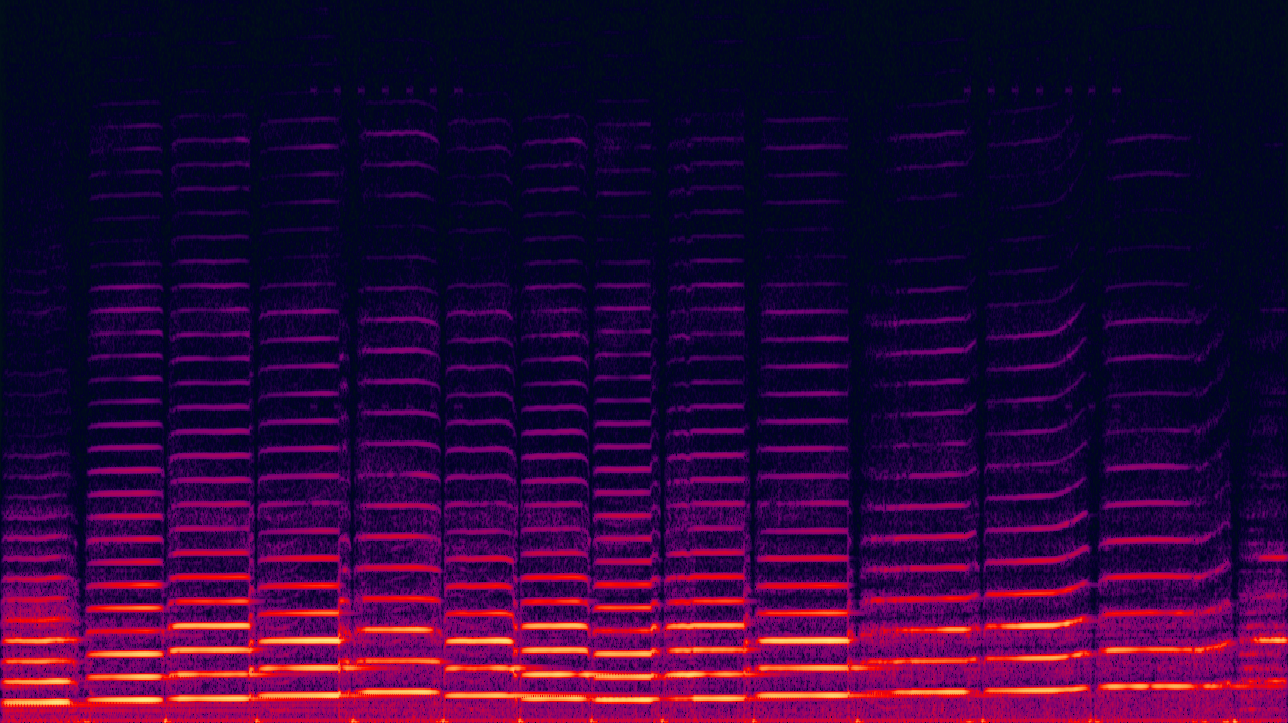
\includegraphics[width=0.8\linewidth]{Figures/Spectrogram.png}
	\caption[Spectogram of a file audio]{Spectogram di un file audio. Immagine di proprietà di \url{https://en.wikipedia.org/wiki/User:Omegatron}, utilizzata sotto licenza Creative Commons Attribution-Share Alike 3.0 Unported (CC BY-SA 3.0) \url{https://creativecommons.org/licenses/by-sa/3.0/deed.en}.}
\end{figure}

\noindent Si può anche valutare l'idea di applicare il metodo di confronto con clustering su opere letterarie, dove l'input è ottenuto come output di un Word Embeddings ossia di un algoritmo che trasforma un testo in una sequenza di vettori considerandone la vicinanza semantica. Questo permette di migliorare il preprocessing e non solo, anche di renderlo parte dell'algoritmo tramite un trasformer preaddestrato che riesce a rilevare sempre più in profondità significati semantici complessi da grandi porzioni di testo.

\noindent Rimanendo nel contesto di questa tesi sarebbe interessante valutare le prestazioni di attribuzione su immagini a colori oppure immagini naturalmente grige ma con dei disegni e non delle sole grafie. Inoltre potrebbero essere usate diverse scale di colori, magari confrontare \gls{rgb} con \gls{hsl} oppure usare scale logaritmiche dei grigi, che possono ben separare i cluster tra di loro.

\noindent Un'altra idea interessante per cambiare il tipo di input su delle immagini è usare le curve di Peano. Questa tecnica non è in realtà così originale, già è stata esplorata per esaminare delle immagini con dei trasformatori (che tipicamente lavorano su sequenze unidimensionali). In particolare l'immagine viene trasformata in una lunga linea di pixel grigi che rappresenta la curva di peano. A questo punto basterà applicare l'algoritmo su questa linea come se fosse una sequenza di lettere.

\subsection{\gls{cada} with \gls{gmm}}
Come già ricordato, in questa tesi si è vista una generalizzazione di \gls{dada} con \gls{cada} applicato a \gls{kmeans} e \gls{fcm}. E' stato anche accennato il clustering \gls{gmm}, il quale però ha una natura completamente diversa da \gls{fcm}. Può essere interessante affrontare comunque questo tipo di clusterizzazione per confrontare due opere. Infatti il clustering \gls{gmm} vuole approssimare la densità ignota originale dei set di samples con una nota. Come spiegato in \cref{chap:LiteratureReview}, dato un set di samples $A$, il clustering \gls{gmm} cercherà i parametri $p_i\in \mathbb{R}$, $\Sigma_i\in\mathbb{R}^{K\times K}$, $\mu_i\in\mathbb{R}^K$ per ogni centroide $i$ che meglio spiegano il set $A$ come originato dal seguente processo:
\begin{enumerate}
	\item Scelgo un centroide $i$ con probabilità $p_i$
	\item Pesco il sample da $\mathcal{N}\left(\mu_i,\Sigma_i\right)$
\end{enumerate}
di conseguenza la densità che approssima $A$ sarà:
\[
	f(x) = \sum_i p_i\phi_i(x)
\]
dove $\phi_i(x)$ è la densità in $x$ della gaussiana multivariata $i$-esima:
\[
	\phi_i(x) = \left(2\pi\right)^{-k/2}\det\left(\Sigma_i\right)^{-1/2}\exp\left(-\frac12\left(x-\mu_i\right)^T\Sigma^{-1}\left(x-\mu_i\right)\right)
\]

Quindi in \cref{eq:SapAttribution_dist} si può chiamare $f_{A}(x)$ la densità che \gls{gmm} propone come approssimazione del set di samples $A$, stessa cosa anche per $B$. Naturalmente si potrà riscrivere la funzione di comparazione tra due samples:
\[
d(A,B)=(1+J_{D_A, D_B})^{-1} \times \int dx\left(\frac{f_A(x)-f_B(x)}{f_A(x)+f_B(x)}\right)^2
\]
Si fa notare che l'indice di Jaccard non è chiaro come definirlo nel contesto di \gls{cada} con \gls{gmm}. Tuttavia dal momento che ci sono delle densità esplicite in gioco potrebbe essere interessante vedere se è possibile fornire una stima numerica molto precisa per questo integrale. E' senz'altro una sfida teorica molto stimolante.

\subsection{Understand the author}
Una analisi che non è stata effettuata è la ricerca di quali tessere hanno maggiormente giustificato il risultato di un confronto. Poiché il metodo \gls{cada} costruisce dei cluster e su questa base dà più peso ai cluster meno rappresentati, sarebbe interessante approfondire il concetto di peso di una tessera ed evidenziare queste tessere nelle due immagini confrontate.

\noindent In particolare da \cref{eq:fuzzy_distance} si considera ideale e fissata la clusterizzazione \gls{fcm} e si fornisce un peso ad ogni centroide $c$. Di conseguenza si potrebbe far ereditare alle tessere il peso del centroide in funzione della membership. L'aspettativa è che le tessere che coinvolgono maggiormente la scrittura dell'autore sono le più coinvolte.

\noindent Altre analisi utili sono ad esempio lo studio dei centroidi, alla ricerca di centroidi tipici dell'autore considerato. Questo permette di formulare nuove tipi di comparazioni basate sui centroidi.

\subsection{Attribution}
Un punto che si fa notare è che i risultati di questa tesi si sono espressi in termini di capacità di attribuzione. Tuttavia in questo elaborato non sono state visionate tecniche di attribuzione, bensì ne è stata usata solo una e anche piuttosto elementare. Potrebbe essere una analisi utile, quella di vedere quali opere di ogni autore hanno caratterizzato di più l'attribuzione. Ad esempio: un'opera che più di tutte ha fornito veri positivi per il suo autore. Questo non solo migliora l'attribuzione, ma la velocizza e fornisce informazioni utili sull'autore.

\noindent Un altro metodo per velocizzare l'analisi è vedere la relazione che vi è tra il valore di comparazione tra due opere e una distanza. Anche se, a giudicare dalla sua definizione in \cref{eq:SapAttribution_dist} non sembra essere una distanza, è possibile che esista un upper bound per il valore di comparazione tra $2$ opere conoscendo le altre comparazioni? In altri termini, se sappiamo che $d(A,B)$ e $d(B,C)$ sono molto piccoli ha senso presumere che anche $d(A,C)$ sarà altrettanto piccolo? Anche solo poter dire (ad esempio) che $d(A,B)+d(B,C) \geq d(A,C)^\frac12$ può significare molto per velocizzare il calcolo nelle attribuzioni.

\subsection{Neural Networks}
Un altro tipo di analisi è comparare il metodo \gls{cada} con le reti neurali. Infatti una semplice rete convoluzionale seguita da un Multi Layer Perceptron (MLP) esamina le immagini in modo molto simile. In primis, entrambi i modelli esaminano piccole tessere estratte dall'immagine, in secundis, entrambi i modelli applicano un clustering per fornire l'output finale. Anche se il calcolo esplicito è molto diverso le idee che ci sono dietro sono molto simili. Sarebbe interessante vedere come collegare i due modelli ed eventualmente trovarne una sinergia nelle applicazioni.

\section{Conclusions}
